\chapter{Centrales térmicas de carbón.}
\section{Esquema funcional de una central de carbón.}
Todas las centrales de combustible fósil clásicas tienen un esquema de funcionamiento prácticamente idéntico con las únicas diferencias siendo:
\begin{itemize}
	\item [-] El tratamiento previo del combustible.
	\item [-] El diseño de los quemadores.
	\item [-] El sistema de limpieza de humos y evacuación de las cenizas.
\end{itemize} 


Pese a ello, en la mayoría de centrales se pueden distinguir los siguientes circuitos básicos:
\begin{itemize}
	\item [-] Circuito de combustión.
	\item [-] Circuito aire-gases.
	\item [-] Circuito agua-vapor.
	\item [-] Circuito de agua de circulación.
	\item [-] Circuitos eléctricos.
	\item [-] Circuitos auxiliares.
\end{itemize}


\begin{figure}[H]
	\centering
	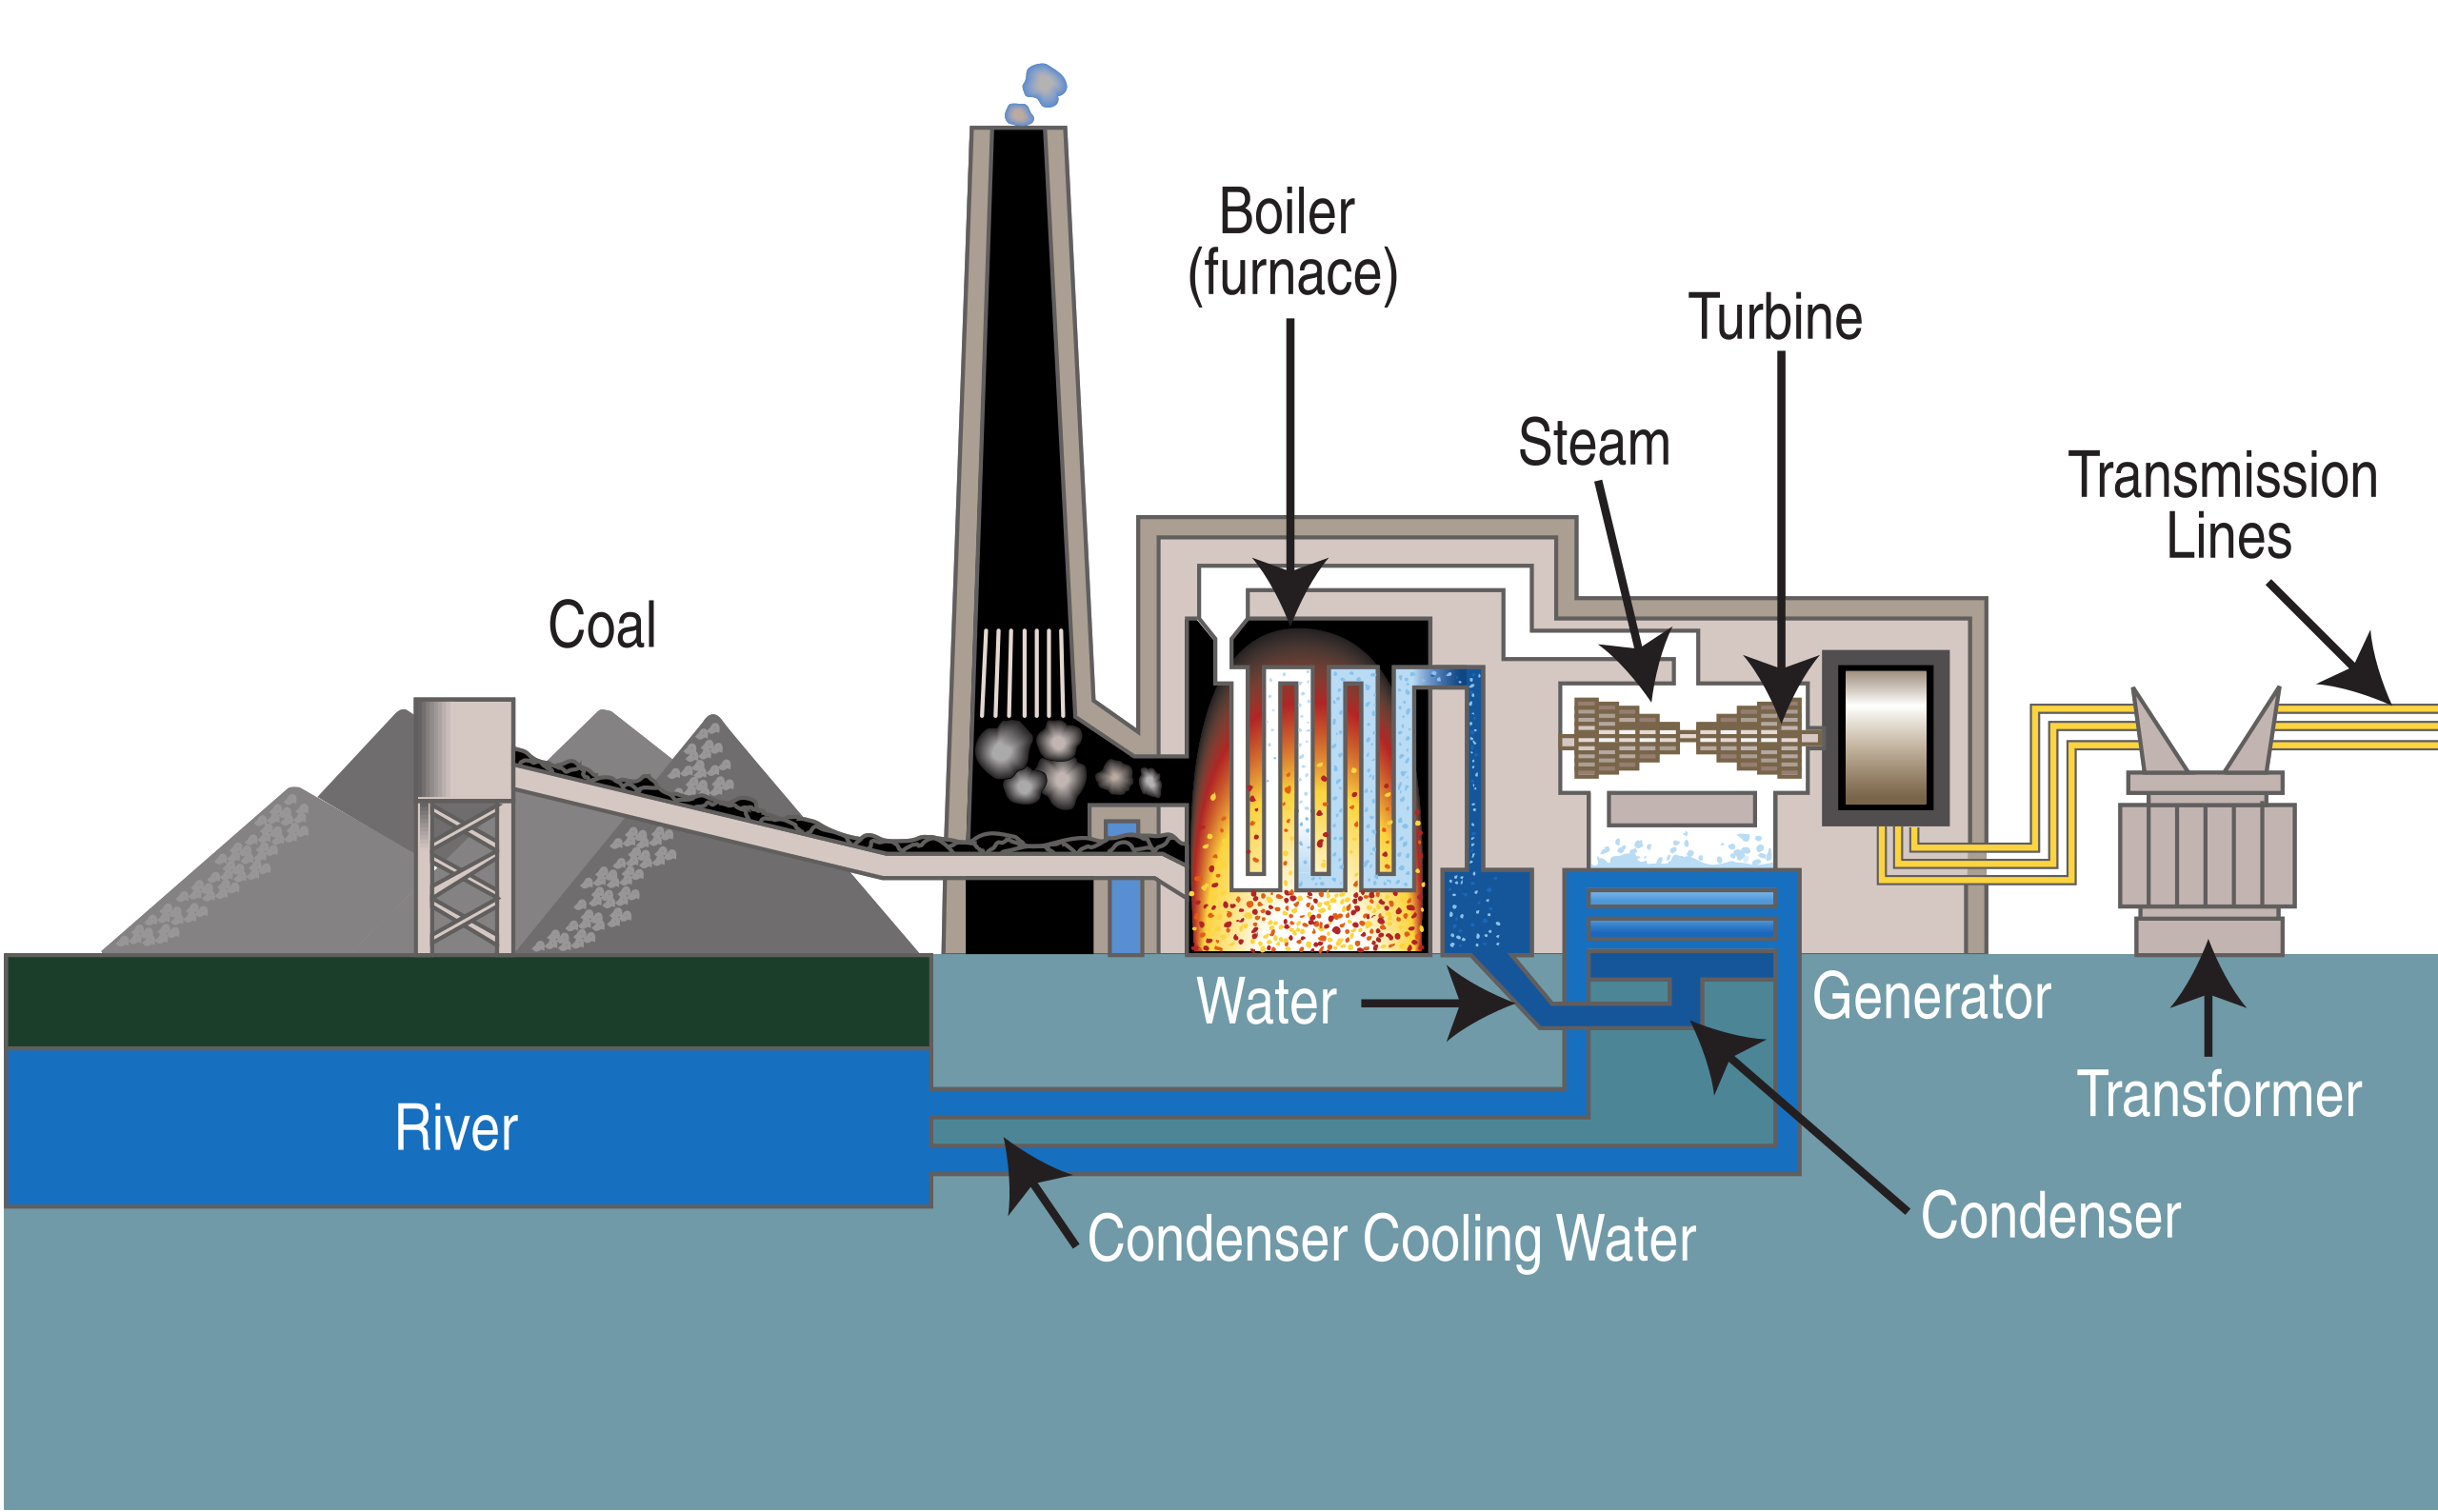
\includegraphics[width=0.7\linewidth]{res/tema10/esquemaFuncional}
	\label{fig:esquemafuncional}
\end{figure}

\section{Circuito aire-combustible-gases-ceniza.}
Este circuito se encarga de:
\begin{itemize}
	\item [-] Recibir y almacenar el combustible.
	\item [-] Preparar el combustible para ser quemado.
	\item [-] Transportar el combustible hasta el hogar.
	\item [-] Evacuación y filtrado de gases.
\end{itemize}
\section{Almacenamiento y preparación del combustible.}
\subsection{Almacenamiento del combustible.}
El almacenamiento se realiza en dos etapas. La primera etapa es el parque de combustible que suele tener una capacidad de almacenamiento de algunos meses de funcionamiento mientras que la segunda se compone por unos depósitos con capacidad para menos de un día.



El carbón se almacena en la cercanía de la central en parques a la intemperie y se maneja mediante rotopalas. Como se debe garantizar que haya un suministro esta la capacidad de almacenamiento suele ser elevada (hasta 150 días). Y si el carbón debe almacenarse más de un año se le proporciona un recubrimiento asfáltico.



No obstante, el almacenamiento de carbón presenta tres problemas principales:
\begin{itemize}
	\item [-] Combustión espontánea: debido al contacto con el aire el carbón se oxida a una velocidad proporcional a la temperatura (se duplica cada 8\grado). A los 65\grado $\ $ empieza a ser peligrosa y por tanto, el apilamiento debe hacerse de manera cuidadosa.
	\item [-] Pérdida de poder calorífica.
	\item [-] Degradación del tamaño del grano.
\end{itemize}


Del parque de almacenamiento se lleva el carbón a una torre de almacenamiento donde se separan las partículas férricas y trozos de piedras que pudiesen dañar los molinos. Tras pasar por la torre el carbón cae a través de las tolvas a unos alimentadores que dosifican la carga a los molinos.
\subsection{Preparación del combustible}
Una parte fundamental de la preparación del combustible consiste en pulverizar el carbón. 



Ventajas de la pulverización:
\begin{itemize}
	\item [-] Rendimiento de la combustión máximo.
	\item [-] Se pueden utilizar carbones de peor calidad.
	\item [-] Las cenizas y escorias no son pastosas (mejor manejo).
	\item [-] Mayor potencia calorífica por unidad de volumen del hogar. 
	\item [-] Menor costo de mano de obra.
 	\item [-] Fácil control del aire y combustible.
\end{itemize}





Desventajas de la pulverización:
\begin{itemize}
	\item [-] Elevado costo inicial de la instalación.
	\item [-] Costo de preparación del combustible.
	\item [-] Posibilidad de crear cenizas volantes (escapen por la chimenea).
\end{itemize}




Además, si el contenido de humedad es muy elevado el carbón antes de entrar al molino se mezcla con gas caliente para evaporar el agua.



Los molinos suelen transformar el carbón desde una granulometría menor a 150 mm hasta un grado de finura de aproximadamente 200$\mu m$ que depende del contenido en volátiles (a mayor contenido en volátiles mayor finura se requiere).



Una vez pulverizado la inyección puede ser:
\begin{itemize}
	\item [-] \textbf{Directa}: el carbón que sale de los molinos se lleva directamente a los quemadores. Es el método \textbf{más utilizado}.
	\item [-] \textbf{Indirecta}: el carbón se hace llegar a los molinos donde es transportado a unos silos de carbón pulverizado donde se almacena hasta que es inyectado en los quemadores.
\end{itemize}
\section{Tipos de molinos.}

\subsection{Molino de anillo de bolas.}
Es un tipo de molino donde un collar de esferas macizas de acero es arrastrado rondado entre dos anillos en los que hay talladas pistas troncotoroidales que guían a las bolas. La presión entre las bolas y anillos se mantiene mediante muelles de acero con una presión regulable.
\begin{figure}[H]
	\centering
	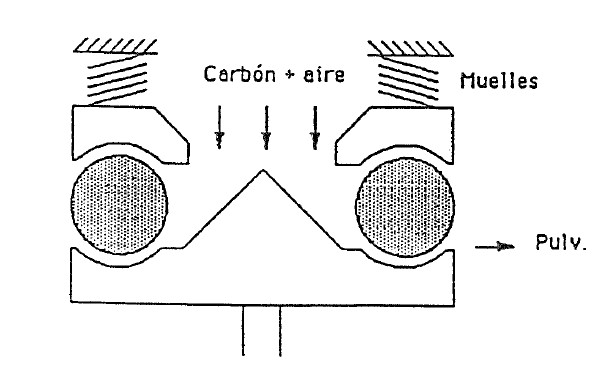
\includegraphics[width=0.4\linewidth]{res/tema10/molinoBolas}
	\label{fig:molinobolas}
\end{figure}

\subsection{Molino tubular de bolas tipo Hardinge.}
Es un molino que consta de un cilindro horizontal con bolas de acero en su interior que gira a velocidad constante. Se emplea aire caliente para secar el carbón y arrastrar el carbón pulverizado a un clasificador espiral.



Como las bolas se van desgastando con el tiempo ne van añadiendo en proporción 0,04-0,23 kg por tonelada de carbón pulverizado. Es un molino adecuado para antracitas aunque es ruidoso y es difícil controlar la finura del polvo. 



Estas calderas suelen absorber de 11 a 30$\frac{kWh}{ton}$ y pueden almacenar grandes cantidades de carbón para seguir suministrando carbón de 6 a 10 minutos.
\begin{figure}[H]
	\centering
	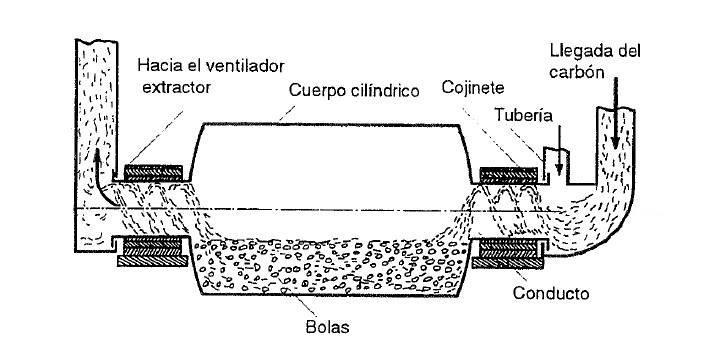
\includegraphics[width=0.6\linewidth]{res/tema10/molinoHardinge}
	\label{fig:molinohardinge}
\end{figure}

\subsection{Molino tubular de bolas Foster Wheeler.}
Es un molino muy simple, adecuado para antracitas. Es ruidoso y de velocidad limitada, pero permite controlar muy bien la finura de polvo. Puede almacenar gran cantidad de carbón.
\begin{figure}[H]
	\centering
	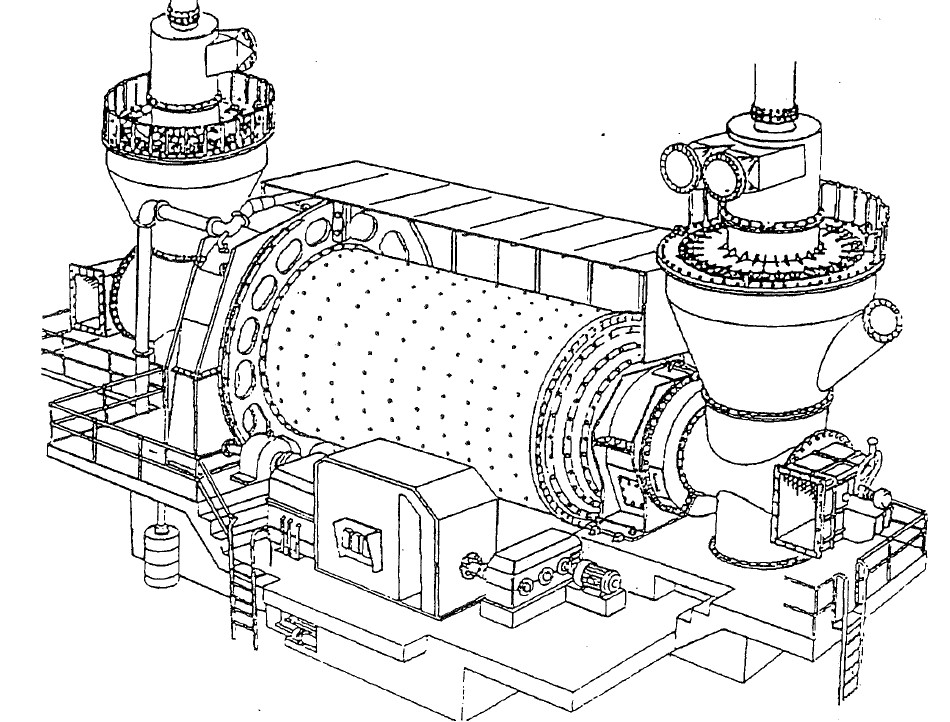
\includegraphics[width=0.4\linewidth]{res/tema10/fosterWheeler}
	\label{fig:fosterwheeler}
\end{figure}

\subsection{Molino de rodillos Babcock-Wilcox.}
Las bolas tienen un diámetro de 51 mm y su velocidad lineal es de 6$\frac{m}{s}$. El consumo de energía es de 8 a 12$\frac{kWh}{ton}$.
\begin{figure}[H]
	\centering
	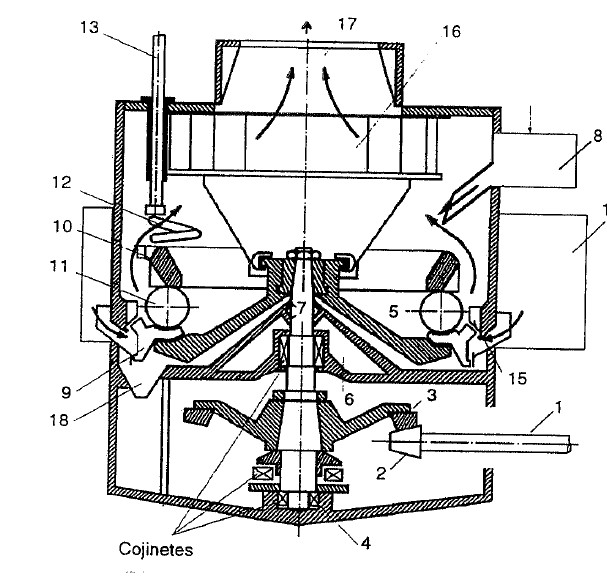
\includegraphics[width=0.3\linewidth]{res/tema10/babcock}
	\label{fig:babcock}
\end{figure}

\subsection{Molino de rodillos de Raymond.}
Este molino consta de tres rodillos que giran sobre un camino de rodadura. La presión correcta se consigue mediante unos muelles ajustables.


Tiene un bajo coste de mantenimiento y es silencioso. Puede triturar 70$\frac{t}{h}$ de carbón pulverizado. Absorbe entre 11 y 16$\frac{kWh}{ton}$.
\begin{figure}[H]
	\centering
	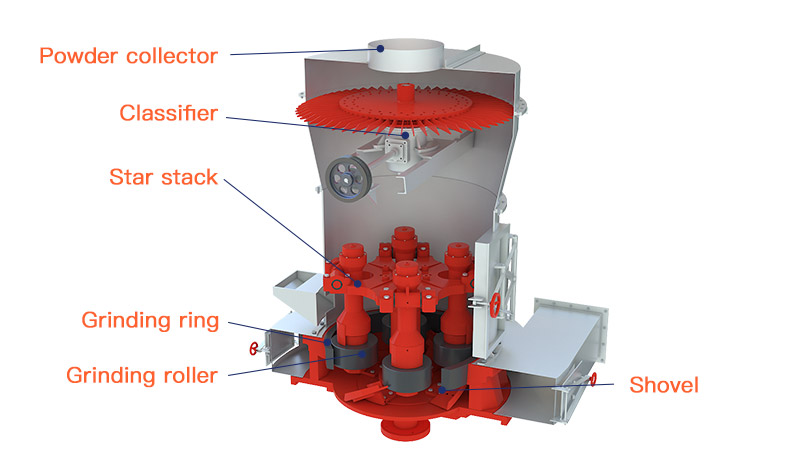
\includegraphics[width=0.5 \linewidth]{res/tema10/raymond}
	\label{fig:raymond}
\end{figure}

\subsection{Molino de batea móvil.}
Es un molino  con una batea móvil con forma troncocónica que gira alrededor de un eje vertical a una velocidad entre 65 y 100 rpm. En su interior se alojan tres muelas cónicas tangentes a la superficie de la batea que giran solidariamente entre sí.




El carbón entra por el centro en el espacio que dejan libres las muelas que a través de la fuerza centrífuga es lanzado contra las paredes donde es triturado por las muelas.


Para extraer este carbón, se emplea aire precalentado que arrastra el carbón pulverizado hacia un separador y las partículas gruesas vuelven al molino.


Este molino tiene bajo costo de mantenimiento y bajo consumo de energía.

\begin{figure}[H]
	\centering
	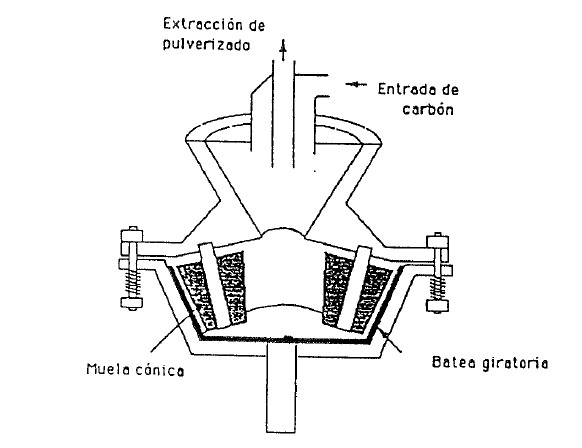
\includegraphics[width=0.5\linewidth]{res/tema10/bateaMovil}
	\label{fig:bateamovil}
\end{figure}


\subsection{Molinos de tipo impacto.}
Este tipo de molinos emplea anillos cilíndricos que giran a una velocidad entre 1000 y 2000 rpm. Dos de los anillos son trituradores y otros dos son lisos para arrastrar el carbón.


A diferencia de anteriores molinos, el carbón descarga directamente por la parte inferior a través de una parrilla que asegura la granulometría deseada.
\begin{figure}[H]
	\centering
	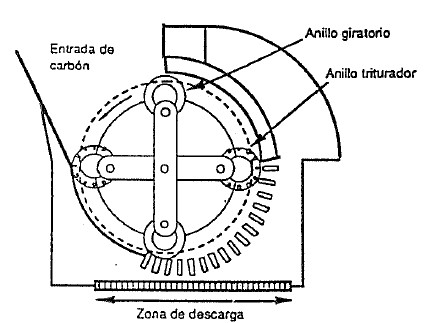
\includegraphics[width=0.5\linewidth]{res/tema10/impacto}
	\label{fig:impacto}
\end{figure}

\section{Circuito aire-gases.}
El aire tomado de la atmósfera se envía mediante ventiladores de tiro forzado a través de precalentadores.

El objetivo de los quemadores:
\begin{itemize}
	\item [-] Recuperar el calor contenido en los gases a la salida de los intercambiadores de agua y vapor.
	\item [-] Elevar la temperatura del aire empleado en la combustión para mejorarla y, para secar el carbón.
\end{itemize}


A la salida de los precalentadores, el aire se envía a la cámara de combustión de diferentes manera:
\begin{itemize}
	\item [-] A través de los quemadores como aire primario mezclado con el combustible.
	\item [-] Alrededor de los quemadores como aire secundario.
	\item [-] A lo largo del recorrido de la llama como aire terciario.
\end{itemize}

\begin{figure}[H]
	\centering
	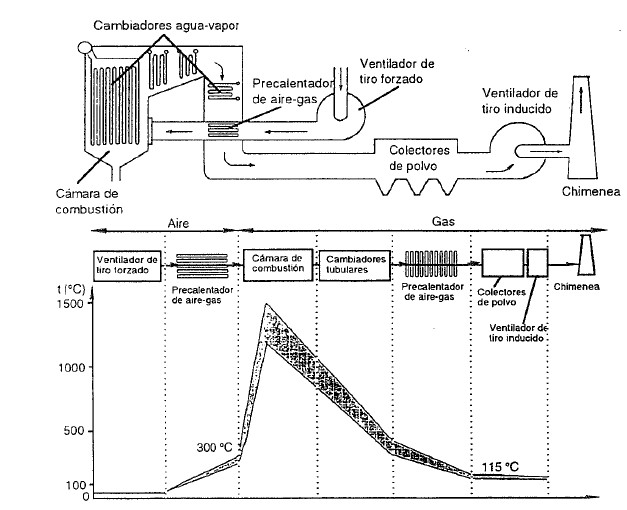
\includegraphics[width=0.7\linewidth]{res/tema10/circuitoAwaGas}
	\label{fig:circuitoawagas}
\end{figure}

\section{Quemadores.}
Los mecheros o quemadores son dispositivos mediante los cuales se introduce carbón pulverizado en suspensión en el aire primario hacia el hogar. Estos dispositivos deben permitir:
\begin{itemize}
	\item [-] El ajuste del punto de ignición.
	\item [-] La estabilidad de la llama (la velocidad de la mezcla aire-carbón iguala a la de propagación de la llama).
	\item [-] La combustión completa.
 	\item [-] La distribución uniforme del exceso de aire y de la temperatura.
	\item [-] El fácil acceso para el mantenimiento.
\end{itemize}



Los quemadores constan de varios conductores donde uno es para el fuel (precalentar el hogar), otro es para el carbón y aire primario y uno adicional para el aire secundario. Además, los quemadores son orientables y se puede modificar su ángulo de incidencia para el control de la combustión.
\begin{figure}[H]
	\centering
	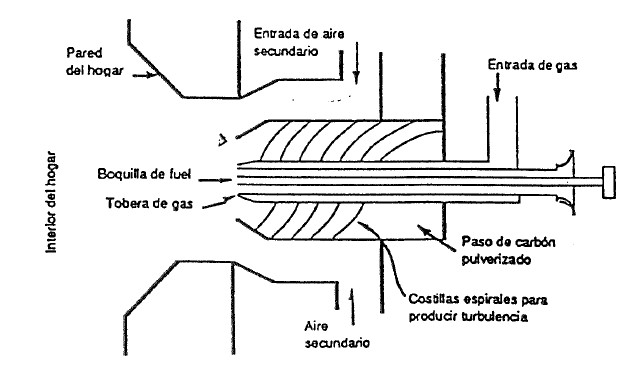
\includegraphics[width=0.6\linewidth]{res/tema10/boquilla}
	\label{fig:boquilla}
\end{figure}


En función del tipo de flujo se tienen:
\begin{itemize}
	\item [-] \textbf{Quemadores de tipo laminar}: las turbulencias se producen por la propia velocidad de la muestra, por el uso de deflectores y por la entrada de aire secundario y terciario.
	\item [-] \textbf{Quemadores de turbulencias}: se imprime un movimiento rotativo al flujo de carbón y aire primario.
\end{itemize}


Para precalentar el hogar de la caldera se emplea combustible líquido (fuel-oil).
\section{Hogar.}
Es la parte de la caldera donde tiene lugar la combustión. El calor desprendido se transmite primero por radiación a todas las partes que están en presencia de la llama y, posteriormente a las partes de la caldera que no ven el fuego mediante convección denominada zona de recuperación de calor (camino de salida de los humos).
\subsection{Pantallas evaporadoras.}
El hogar de una caldera es un volumen diáfano de grandes dimensiones cuyas paredes están
constituidas habitualmente por paneles verticales de tubos soldados de aletas longitudinales
(pantallas evaporadoras). Normalmente van dispuestos verticalmente, soldados a los colectores
extremos (entrada inferior y salida superior).




Por el interior de estos paneles asciende agua de alimentación precalentada a 100\grado $\ $ procedente del economizador, a través de tubos recubiertos de materiales refractarios que bajan desde la parte superior de la caldera (downcommers) que actúa como fluido refrigerante de los propios tubos.


Las paredes de agua van fijas a la envolvente de la caldera de modo que permita su libre
dilatación. 


La envolvente de la caldera es chapa metálica mientras el aislamiento térmico de las paredes
es cemento refractario o roca de vidrio
\section{Ventiladores.}
Para regular la presión en el interior del hogar se emplean ventiladores de tiro forzado que impulsan el aire al interior del hogar para proporcionar presión suficiente para vencer las pérdidas de carga en el circuito aire-gas. No obstante, si la presión en el interior del hogar es menor a la atmosférica (depresión) es necesario un segundo ventilador, de tiro inducido, para aspirar los gases de la combustión y enviarlos a la chimenea.



Las calderas de combustible sólido suelen estar en depresión y las de combustibles líquidos o gaseosos son presurizados.
\subsection{Ventiladores de tiro forzado.}
Se introduce aire a presión al hogar de forma que se vencen los rozamientos y las pérdidas de carga en todo el recorrido de los gases de combustión.
\begin{figure}[H]
	\centering
	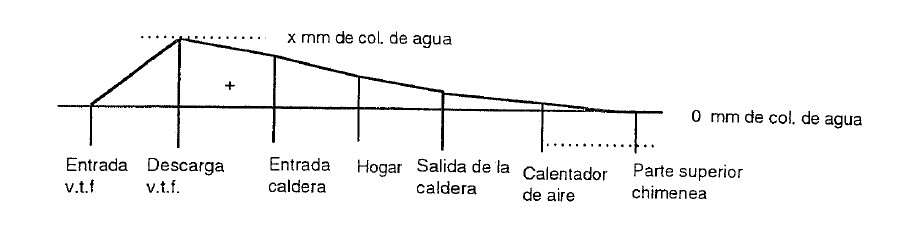
\includegraphics[width=0.7\linewidth]{res/tema10/forzao}
	\label{fig:forzao}
\end{figure}

\subsection{Ventiladores de tiro inducido.}
Se colocan dos por seguridad y se encargan de aspirar los gases del hogar y los envían a la chimenea.
\begin{figure}[H]
	\centering
	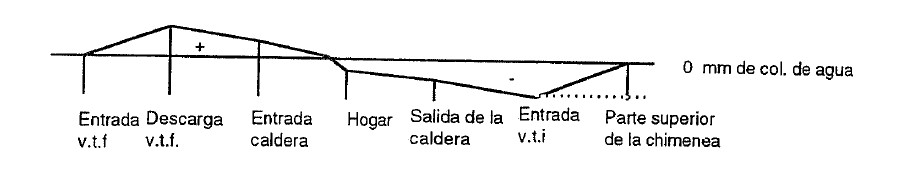
\includegraphics[width=0.7\linewidth]{res/tema10/inducio}
	\label{fig:inducio}
\end{figure}

\section{Precalentadores.}
f
\section{Productos de desecho.}
f
\section{Ceniceros.}
f
\section{Retención de cenizas.}
f
\section{Chimenea.}
f
\section{Circuito agua vapor.}
f
\section{Ciclo de Rankine.}
f
\section{Caldera acuotubular.}
f
\section{Calderín.}
f
\section{Sobrecalentadores.}
f
\section{Economizador.}
f
\section{Líneas de vapor.}
f
\section{Turbinas de vapor.}
f
\section{Condensadores.}
f
\section{Desgasificador.}
f
\section{Sistema de refrigeración.}
f
\section{Control.}
f